
% Default to the notebook output style

    


% Inherit from the specified cell style.




    
\documentclass[11pt]{article}

    
    
    \usepackage[T1]{fontenc}
    % Nicer default font (+ math font) than Computer Modern for most use cases
    \usepackage{mathpazo}

    % Basic figure setup, for now with no caption control since it's done
    % automatically by Pandoc (which extracts ![](path) syntax from Markdown).
    \usepackage{graphicx}
    % We will generate all images so they have a width \maxwidth. This means
    % that they will get their normal width if they fit onto the page, but
    % are scaled down if they would overflow the margins.
    \makeatletter
    \def\maxwidth{\ifdim\Gin@nat@width>\linewidth\linewidth
    \else\Gin@nat@width\fi}
    \makeatother
    \let\Oldincludegraphics\includegraphics
    % Set max figure width to be 80% of text width, for now hardcoded.
    \renewcommand{\includegraphics}[1]{\Oldincludegraphics[width=.8\maxwidth]{#1}}
    % Ensure that by default, figures have no caption (until we provide a
    % proper Figure object with a Caption API and a way to capture that
    % in the conversion process - todo).
    \usepackage{caption}
    \DeclareCaptionLabelFormat{nolabel}{}
    \captionsetup{labelformat=nolabel}

    \usepackage{adjustbox} % Used to constrain images to a maximum size 
    \usepackage{xcolor} % Allow colors to be defined
    \usepackage{enumerate} % Needed for markdown enumerations to work
    \usepackage{geometry} % Used to adjust the document margins
    \usepackage{amsmath} % Equations
    \usepackage{amssymb} % Equations
    \usepackage{textcomp} % defines textquotesingle
    % Hack from http://tex.stackexchange.com/a/47451/13684:
    \AtBeginDocument{%
        \def\PYZsq{\textquotesingle}% Upright quotes in Pygmentized code
    }
    \usepackage{upquote} % Upright quotes for verbatim code
    \usepackage{eurosym} % defines \euro
    \usepackage[mathletters]{ucs} % Extended unicode (utf-8) support
    \usepackage[utf8x]{inputenc} % Allow utf-8 characters in the tex document
    \usepackage{fancyvrb} % verbatim replacement that allows latex
    \usepackage{grffile} % extends the file name processing of package graphics 
                         % to support a larger range 
    % The hyperref package gives us a pdf with properly built
    % internal navigation ('pdf bookmarks' for the table of contents,
    % internal cross-reference links, web links for URLs, etc.)
    \usepackage{hyperref}
    \usepackage{longtable} % longtable support required by pandoc >1.10
    \usepackage{booktabs}  % table support for pandoc > 1.12.2
    \usepackage[inline]{enumitem} % IRkernel/repr support (it uses the enumerate* environment)
    \usepackage[normalem]{ulem} % ulem is needed to support strikethroughs (\sout)
                                % normalem makes italics be italics, not underlines
    

    
    
    % Colors for the hyperref package
    \definecolor{urlcolor}{rgb}{0,.145,.698}
    \definecolor{linkcolor}{rgb}{.71,0.21,0.01}
    \definecolor{citecolor}{rgb}{.12,.54,.11}

    % ANSI colors
    \definecolor{ansi-black}{HTML}{3E424D}
    \definecolor{ansi-black-intense}{HTML}{282C36}
    \definecolor{ansi-red}{HTML}{E75C58}
    \definecolor{ansi-red-intense}{HTML}{B22B31}
    \definecolor{ansi-green}{HTML}{00A250}
    \definecolor{ansi-green-intense}{HTML}{007427}
    \definecolor{ansi-yellow}{HTML}{DDB62B}
    \definecolor{ansi-yellow-intense}{HTML}{B27D12}
    \definecolor{ansi-blue}{HTML}{208FFB}
    \definecolor{ansi-blue-intense}{HTML}{0065CA}
    \definecolor{ansi-magenta}{HTML}{D160C4}
    \definecolor{ansi-magenta-intense}{HTML}{A03196}
    \definecolor{ansi-cyan}{HTML}{60C6C8}
    \definecolor{ansi-cyan-intense}{HTML}{258F8F}
    \definecolor{ansi-white}{HTML}{C5C1B4}
    \definecolor{ansi-white-intense}{HTML}{A1A6B2}

    % commands and environments needed by pandoc snippets
    % extracted from the output of `pandoc -s`
    \providecommand{\tightlist}{%
      \setlength{\itemsep}{0pt}\setlength{\parskip}{0pt}}
    \DefineVerbatimEnvironment{Highlighting}{Verbatim}{commandchars=\\\{\}}
    % Add ',fontsize=\small' for more characters per line
    \newenvironment{Shaded}{}{}
    \newcommand{\KeywordTok}[1]{\textcolor[rgb]{0.00,0.44,0.13}{\textbf{{#1}}}}
    \newcommand{\DataTypeTok}[1]{\textcolor[rgb]{0.56,0.13,0.00}{{#1}}}
    \newcommand{\DecValTok}[1]{\textcolor[rgb]{0.25,0.63,0.44}{{#1}}}
    \newcommand{\BaseNTok}[1]{\textcolor[rgb]{0.25,0.63,0.44}{{#1}}}
    \newcommand{\FloatTok}[1]{\textcolor[rgb]{0.25,0.63,0.44}{{#1}}}
    \newcommand{\CharTok}[1]{\textcolor[rgb]{0.25,0.44,0.63}{{#1}}}
    \newcommand{\StringTok}[1]{\textcolor[rgb]{0.25,0.44,0.63}{{#1}}}
    \newcommand{\CommentTok}[1]{\textcolor[rgb]{0.38,0.63,0.69}{\textit{{#1}}}}
    \newcommand{\OtherTok}[1]{\textcolor[rgb]{0.00,0.44,0.13}{{#1}}}
    \newcommand{\AlertTok}[1]{\textcolor[rgb]{1.00,0.00,0.00}{\textbf{{#1}}}}
    \newcommand{\FunctionTok}[1]{\textcolor[rgb]{0.02,0.16,0.49}{{#1}}}
    \newcommand{\RegionMarkerTok}[1]{{#1}}
    \newcommand{\ErrorTok}[1]{\textcolor[rgb]{1.00,0.00,0.00}{\textbf{{#1}}}}
    \newcommand{\NormalTok}[1]{{#1}}
    
    % Additional commands for more recent versions of Pandoc
    \newcommand{\ConstantTok}[1]{\textcolor[rgb]{0.53,0.00,0.00}{{#1}}}
    \newcommand{\SpecialCharTok}[1]{\textcolor[rgb]{0.25,0.44,0.63}{{#1}}}
    \newcommand{\VerbatimStringTok}[1]{\textcolor[rgb]{0.25,0.44,0.63}{{#1}}}
    \newcommand{\SpecialStringTok}[1]{\textcolor[rgb]{0.73,0.40,0.53}{{#1}}}
    \newcommand{\ImportTok}[1]{{#1}}
    \newcommand{\DocumentationTok}[1]{\textcolor[rgb]{0.73,0.13,0.13}{\textit{{#1}}}}
    \newcommand{\AnnotationTok}[1]{\textcolor[rgb]{0.38,0.63,0.69}{\textbf{\textit{{#1}}}}}
    \newcommand{\CommentVarTok}[1]{\textcolor[rgb]{0.38,0.63,0.69}{\textbf{\textit{{#1}}}}}
    \newcommand{\VariableTok}[1]{\textcolor[rgb]{0.10,0.09,0.49}{{#1}}}
    \newcommand{\ControlFlowTok}[1]{\textcolor[rgb]{0.00,0.44,0.13}{\textbf{{#1}}}}
    \newcommand{\OperatorTok}[1]{\textcolor[rgb]{0.40,0.40,0.40}{{#1}}}
    \newcommand{\BuiltInTok}[1]{{#1}}
    \newcommand{\ExtensionTok}[1]{{#1}}
    \newcommand{\PreprocessorTok}[1]{\textcolor[rgb]{0.74,0.48,0.00}{{#1}}}
    \newcommand{\AttributeTok}[1]{\textcolor[rgb]{0.49,0.56,0.16}{{#1}}}
    \newcommand{\InformationTok}[1]{\textcolor[rgb]{0.38,0.63,0.69}{\textbf{\textit{{#1}}}}}
    \newcommand{\WarningTok}[1]{\textcolor[rgb]{0.38,0.63,0.69}{\textbf{\textit{{#1}}}}}
    
    
    % Define a nice break command that doesn't care if a line doesn't already
    % exist.
    \def\br{\hspace*{\fill} \\* }
    % Math Jax compatability definitions
    \def\gt{>}
    \def\lt{<}
    % Document parameters
    \title{dinsta-ria1}
    
    
    

    % Pygments definitions
    
\makeatletter
\def\PY@reset{\let\PY@it=\relax \let\PY@bf=\relax%
    \let\PY@ul=\relax \let\PY@tc=\relax%
    \let\PY@bc=\relax \let\PY@ff=\relax}
\def\PY@tok#1{\csname PY@tok@#1\endcsname}
\def\PY@toks#1+{\ifx\relax#1\empty\else%
    \PY@tok{#1}\expandafter\PY@toks\fi}
\def\PY@do#1{\PY@bc{\PY@tc{\PY@ul{%
    \PY@it{\PY@bf{\PY@ff{#1}}}}}}}
\def\PY#1#2{\PY@reset\PY@toks#1+\relax+\PY@do{#2}}

\expandafter\def\csname PY@tok@w\endcsname{\def\PY@tc##1{\textcolor[rgb]{0.73,0.73,0.73}{##1}}}
\expandafter\def\csname PY@tok@c\endcsname{\let\PY@it=\textit\def\PY@tc##1{\textcolor[rgb]{0.25,0.50,0.50}{##1}}}
\expandafter\def\csname PY@tok@cp\endcsname{\def\PY@tc##1{\textcolor[rgb]{0.74,0.48,0.00}{##1}}}
\expandafter\def\csname PY@tok@k\endcsname{\let\PY@bf=\textbf\def\PY@tc##1{\textcolor[rgb]{0.00,0.50,0.00}{##1}}}
\expandafter\def\csname PY@tok@kp\endcsname{\def\PY@tc##1{\textcolor[rgb]{0.00,0.50,0.00}{##1}}}
\expandafter\def\csname PY@tok@kt\endcsname{\def\PY@tc##1{\textcolor[rgb]{0.69,0.00,0.25}{##1}}}
\expandafter\def\csname PY@tok@o\endcsname{\def\PY@tc##1{\textcolor[rgb]{0.40,0.40,0.40}{##1}}}
\expandafter\def\csname PY@tok@ow\endcsname{\let\PY@bf=\textbf\def\PY@tc##1{\textcolor[rgb]{0.67,0.13,1.00}{##1}}}
\expandafter\def\csname PY@tok@nb\endcsname{\def\PY@tc##1{\textcolor[rgb]{0.00,0.50,0.00}{##1}}}
\expandafter\def\csname PY@tok@nf\endcsname{\def\PY@tc##1{\textcolor[rgb]{0.00,0.00,1.00}{##1}}}
\expandafter\def\csname PY@tok@nc\endcsname{\let\PY@bf=\textbf\def\PY@tc##1{\textcolor[rgb]{0.00,0.00,1.00}{##1}}}
\expandafter\def\csname PY@tok@nn\endcsname{\let\PY@bf=\textbf\def\PY@tc##1{\textcolor[rgb]{0.00,0.00,1.00}{##1}}}
\expandafter\def\csname PY@tok@ne\endcsname{\let\PY@bf=\textbf\def\PY@tc##1{\textcolor[rgb]{0.82,0.25,0.23}{##1}}}
\expandafter\def\csname PY@tok@nv\endcsname{\def\PY@tc##1{\textcolor[rgb]{0.10,0.09,0.49}{##1}}}
\expandafter\def\csname PY@tok@no\endcsname{\def\PY@tc##1{\textcolor[rgb]{0.53,0.00,0.00}{##1}}}
\expandafter\def\csname PY@tok@nl\endcsname{\def\PY@tc##1{\textcolor[rgb]{0.63,0.63,0.00}{##1}}}
\expandafter\def\csname PY@tok@ni\endcsname{\let\PY@bf=\textbf\def\PY@tc##1{\textcolor[rgb]{0.60,0.60,0.60}{##1}}}
\expandafter\def\csname PY@tok@na\endcsname{\def\PY@tc##1{\textcolor[rgb]{0.49,0.56,0.16}{##1}}}
\expandafter\def\csname PY@tok@nt\endcsname{\let\PY@bf=\textbf\def\PY@tc##1{\textcolor[rgb]{0.00,0.50,0.00}{##1}}}
\expandafter\def\csname PY@tok@nd\endcsname{\def\PY@tc##1{\textcolor[rgb]{0.67,0.13,1.00}{##1}}}
\expandafter\def\csname PY@tok@s\endcsname{\def\PY@tc##1{\textcolor[rgb]{0.73,0.13,0.13}{##1}}}
\expandafter\def\csname PY@tok@sd\endcsname{\let\PY@it=\textit\def\PY@tc##1{\textcolor[rgb]{0.73,0.13,0.13}{##1}}}
\expandafter\def\csname PY@tok@si\endcsname{\let\PY@bf=\textbf\def\PY@tc##1{\textcolor[rgb]{0.73,0.40,0.53}{##1}}}
\expandafter\def\csname PY@tok@se\endcsname{\let\PY@bf=\textbf\def\PY@tc##1{\textcolor[rgb]{0.73,0.40,0.13}{##1}}}
\expandafter\def\csname PY@tok@sr\endcsname{\def\PY@tc##1{\textcolor[rgb]{0.73,0.40,0.53}{##1}}}
\expandafter\def\csname PY@tok@ss\endcsname{\def\PY@tc##1{\textcolor[rgb]{0.10,0.09,0.49}{##1}}}
\expandafter\def\csname PY@tok@sx\endcsname{\def\PY@tc##1{\textcolor[rgb]{0.00,0.50,0.00}{##1}}}
\expandafter\def\csname PY@tok@m\endcsname{\def\PY@tc##1{\textcolor[rgb]{0.40,0.40,0.40}{##1}}}
\expandafter\def\csname PY@tok@gh\endcsname{\let\PY@bf=\textbf\def\PY@tc##1{\textcolor[rgb]{0.00,0.00,0.50}{##1}}}
\expandafter\def\csname PY@tok@gu\endcsname{\let\PY@bf=\textbf\def\PY@tc##1{\textcolor[rgb]{0.50,0.00,0.50}{##1}}}
\expandafter\def\csname PY@tok@gd\endcsname{\def\PY@tc##1{\textcolor[rgb]{0.63,0.00,0.00}{##1}}}
\expandafter\def\csname PY@tok@gi\endcsname{\def\PY@tc##1{\textcolor[rgb]{0.00,0.63,0.00}{##1}}}
\expandafter\def\csname PY@tok@gr\endcsname{\def\PY@tc##1{\textcolor[rgb]{1.00,0.00,0.00}{##1}}}
\expandafter\def\csname PY@tok@ge\endcsname{\let\PY@it=\textit}
\expandafter\def\csname PY@tok@gs\endcsname{\let\PY@bf=\textbf}
\expandafter\def\csname PY@tok@gp\endcsname{\let\PY@bf=\textbf\def\PY@tc##1{\textcolor[rgb]{0.00,0.00,0.50}{##1}}}
\expandafter\def\csname PY@tok@go\endcsname{\def\PY@tc##1{\textcolor[rgb]{0.53,0.53,0.53}{##1}}}
\expandafter\def\csname PY@tok@gt\endcsname{\def\PY@tc##1{\textcolor[rgb]{0.00,0.27,0.87}{##1}}}
\expandafter\def\csname PY@tok@err\endcsname{\def\PY@bc##1{\setlength{\fboxsep}{0pt}\fcolorbox[rgb]{1.00,0.00,0.00}{1,1,1}{\strut ##1}}}
\expandafter\def\csname PY@tok@kc\endcsname{\let\PY@bf=\textbf\def\PY@tc##1{\textcolor[rgb]{0.00,0.50,0.00}{##1}}}
\expandafter\def\csname PY@tok@kd\endcsname{\let\PY@bf=\textbf\def\PY@tc##1{\textcolor[rgb]{0.00,0.50,0.00}{##1}}}
\expandafter\def\csname PY@tok@kn\endcsname{\let\PY@bf=\textbf\def\PY@tc##1{\textcolor[rgb]{0.00,0.50,0.00}{##1}}}
\expandafter\def\csname PY@tok@kr\endcsname{\let\PY@bf=\textbf\def\PY@tc##1{\textcolor[rgb]{0.00,0.50,0.00}{##1}}}
\expandafter\def\csname PY@tok@bp\endcsname{\def\PY@tc##1{\textcolor[rgb]{0.00,0.50,0.00}{##1}}}
\expandafter\def\csname PY@tok@fm\endcsname{\def\PY@tc##1{\textcolor[rgb]{0.00,0.00,1.00}{##1}}}
\expandafter\def\csname PY@tok@vc\endcsname{\def\PY@tc##1{\textcolor[rgb]{0.10,0.09,0.49}{##1}}}
\expandafter\def\csname PY@tok@vg\endcsname{\def\PY@tc##1{\textcolor[rgb]{0.10,0.09,0.49}{##1}}}
\expandafter\def\csname PY@tok@vi\endcsname{\def\PY@tc##1{\textcolor[rgb]{0.10,0.09,0.49}{##1}}}
\expandafter\def\csname PY@tok@vm\endcsname{\def\PY@tc##1{\textcolor[rgb]{0.10,0.09,0.49}{##1}}}
\expandafter\def\csname PY@tok@sa\endcsname{\def\PY@tc##1{\textcolor[rgb]{0.73,0.13,0.13}{##1}}}
\expandafter\def\csname PY@tok@sb\endcsname{\def\PY@tc##1{\textcolor[rgb]{0.73,0.13,0.13}{##1}}}
\expandafter\def\csname PY@tok@sc\endcsname{\def\PY@tc##1{\textcolor[rgb]{0.73,0.13,0.13}{##1}}}
\expandafter\def\csname PY@tok@dl\endcsname{\def\PY@tc##1{\textcolor[rgb]{0.73,0.13,0.13}{##1}}}
\expandafter\def\csname PY@tok@s2\endcsname{\def\PY@tc##1{\textcolor[rgb]{0.73,0.13,0.13}{##1}}}
\expandafter\def\csname PY@tok@sh\endcsname{\def\PY@tc##1{\textcolor[rgb]{0.73,0.13,0.13}{##1}}}
\expandafter\def\csname PY@tok@s1\endcsname{\def\PY@tc##1{\textcolor[rgb]{0.73,0.13,0.13}{##1}}}
\expandafter\def\csname PY@tok@mb\endcsname{\def\PY@tc##1{\textcolor[rgb]{0.40,0.40,0.40}{##1}}}
\expandafter\def\csname PY@tok@mf\endcsname{\def\PY@tc##1{\textcolor[rgb]{0.40,0.40,0.40}{##1}}}
\expandafter\def\csname PY@tok@mh\endcsname{\def\PY@tc##1{\textcolor[rgb]{0.40,0.40,0.40}{##1}}}
\expandafter\def\csname PY@tok@mi\endcsname{\def\PY@tc##1{\textcolor[rgb]{0.40,0.40,0.40}{##1}}}
\expandafter\def\csname PY@tok@il\endcsname{\def\PY@tc##1{\textcolor[rgb]{0.40,0.40,0.40}{##1}}}
\expandafter\def\csname PY@tok@mo\endcsname{\def\PY@tc##1{\textcolor[rgb]{0.40,0.40,0.40}{##1}}}
\expandafter\def\csname PY@tok@ch\endcsname{\let\PY@it=\textit\def\PY@tc##1{\textcolor[rgb]{0.25,0.50,0.50}{##1}}}
\expandafter\def\csname PY@tok@cm\endcsname{\let\PY@it=\textit\def\PY@tc##1{\textcolor[rgb]{0.25,0.50,0.50}{##1}}}
\expandafter\def\csname PY@tok@cpf\endcsname{\let\PY@it=\textit\def\PY@tc##1{\textcolor[rgb]{0.25,0.50,0.50}{##1}}}
\expandafter\def\csname PY@tok@c1\endcsname{\let\PY@it=\textit\def\PY@tc##1{\textcolor[rgb]{0.25,0.50,0.50}{##1}}}
\expandafter\def\csname PY@tok@cs\endcsname{\let\PY@it=\textit\def\PY@tc##1{\textcolor[rgb]{0.25,0.50,0.50}{##1}}}

\def\PYZbs{\char`\\}
\def\PYZus{\char`\_}
\def\PYZob{\char`\{}
\def\PYZcb{\char`\}}
\def\PYZca{\char`\^}
\def\PYZam{\char`\&}
\def\PYZlt{\char`\<}
\def\PYZgt{\char`\>}
\def\PYZsh{\char`\#}
\def\PYZpc{\char`\%}
\def\PYZdl{\char`\$}
\def\PYZhy{\char`\-}
\def\PYZsq{\char`\'}
\def\PYZdq{\char`\"}
\def\PYZti{\char`\~}
% for compatibility with earlier versions
\def\PYZat{@}
\def\PYZlb{[}
\def\PYZrb{]}
\makeatother


    % Exact colors from NB
    \definecolor{incolor}{rgb}{0.0, 0.0, 0.5}
    \definecolor{outcolor}{rgb}{0.545, 0.0, 0.0}



    
    % Prevent overflowing lines due to hard-to-break entities
    \sloppy 
    % Setup hyperref package
    \hypersetup{
      breaklinks=true,  % so long urls are correctly broken across lines
      colorlinks=true,
      urlcolor=urlcolor,
      linkcolor=linkcolor,
      citecolor=citecolor,
      }
    % Slightly bigger margins than the latex defaults
    
    \geometry{verbose,tmargin=1in,bmargin=1in,lmargin=1in,rmargin=1in}
    
    

    \begin{document}
    
    
    \maketitle
    
    

    
    \hypertarget{dinamica-e-stabilituxe0}{%
\section{Dinamica e Stabilità}\label{dinamica-e-stabilituxe0}}

    \hypertarget{sistemi-dinamici}{%
\section{Sistemi dinamici}\label{sistemi-dinamici}}

\hypertarget{introduzione}{%
\subsection{Introduzione}\label{introduzione}}

\hypertarget{definizione-di-sistema}{%
\subsubsection{Definizione di sistema}\label{definizione-di-sistema}}

\begin{quote}
Aggregazione di parti che formano un tutt'uno e che interagisvcono con
il suo ambiente tramite entrate ed uscite
\end{quote}

\hypertarget{siso-vs-mimo}{%
\subsubsection{SISO vs MIMO}\label{siso-vs-mimo}}

SISO = Single Input, Single Output\\
MIMO = Multiple Input, Multiple Output

\hypertarget{proprietuxe0-di-sistema}{%
\subsubsection{Proprietà di sistema}\label{proprietuxe0-di-sistema}}

\hypertarget{statica-vs-dinamica}{%
\paragraph{Statica vs Dinamica}\label{statica-vs-dinamica}}

Statico

\begin{quote}
Il sistema è denominato statico se l'uscita \(y\) al tempo \(t\) dipende
unicamente dal valore dell'entrata \(u\) al tempo \(t\)
\end{quote}

Dinamico

\begin{quote}
Il sistema è dinamico se l'uscita dipende anche dalla ``storia'' passata
del sistema. Il sistema dinamico ha memoria di quello che è successo nel
passato.
\end{quote}

\hypertarget{stato}{%
\paragraph{Stato}\label{stato}}

Anche chiamato ``Condizioni Iniziali''

\begin{quote}
Espresso con un certo numero di variabili. Il numero minimo delle
variabili necessarie per determinare lo stato viene chiamato
\emph{ordine} del sistema
\end{quote}

\hypertarget{invarianza-nel-tempo}{%
\paragraph{Invarianza nel tempo}\label{invarianza-nel-tempo}}

\begin{quote}
Un sistema è \emph{invariante nel tempo} quando l'uscita ottenuta per un
sistema con stato iniziale ed entrata dati è semplicemente traslata nel
tempo se, a partià di stato iniziale, l'entrata del sistema è traslata
nel tempo.
\end{quote}

\begin{equation}
y(t) = f(x_0, u(t))\quad \Longrightarrow \quad y(t-\tau) = f(x_0, u(t-\tau))
\end{equation}

\hypertarget{linearituxe0}{%
\paragraph{Linearità}\label{linearituxe0}}

Un sistema è lineare quando soddisfa la condizione: \begin{equation}
f(\alpha \cdot x + \beta \cdot y) = \alpha \cdot f(x) + \beta \cdot f(y)
\end{equation}

    \hypertarget{modellazione}{%
\subsection{Modellazione}\label{modellazione}}

\hypertarget{mediante-grafi-di-flusso}{%
\subsubsection{Mediante grafi di
flusso}\label{mediante-grafi-di-flusso}}

\hypertarget{rappresentazione}{%
\paragraph{Rappresentazione}\label{rappresentazione}}

\begin{quote}
Per analizzare sistemi \emph{lineari} si possono usare i diagrammi di
flusso di segnali (signal-flow graphs). In questo tipo di
rappresentazione le variabili sono rappresentate da nodi, le dipendenze
lineari tra le variabili da archi diretti pesati.
\end{quote}

Quando il peso di un arco è omesso, esso vale 1.

    \hypertarget{operazioni-sui-diagrammi-di-flusso}{%
\paragraph{Operazioni sui diagrammi di
flusso}\label{operazioni-sui-diagrammi-di-flusso}}

\hypertarget{riduzione-secondo-mason}{%
\subparagraph{Riduzione secondo Mason}\label{riduzione-secondo-mason}}

Percorso

\begin{quote}
Sequenza di linee direzionate che conducono da un nodo ad un altro senza
passare più volte dallo stesso nodo. Il valore di un percorso è il
prodotto del valore di tutte le linee che compongono il percorso.
\end{quote}

    Loop

\begin{quote}
Percorso nel quale il nodo di partenza ed il nodo di arrivo sono
identici. Il valore del loop è il prodotto del valore di tutte le linee
che compongono il loop.
\end{quote}

    Nodo indipendente

Nodo verso il quale non sono puntate linee direzionate.

    Determinante

Il determinante di un diagramma è dato dall'espressione:

\begin{equation}
\Delta = 1 - \sum_i L_i +\sum_{ij} L_i \cdot L_j + \sum_{ijk} L_i \cdot L_j \cdot L_k + \sum_{ijkl} L_i \cdot L_j \cdot L_k \cdot L_l\  +\ ...
\end{equation}

    where:

\begin{itemize}
\tightlist
\item
  \(\sum_i L_i\) is the loop gain of each closed loop in the system,
\item
  \(\sum_{ij} L_i \cdot L_j\) is the product of the loop gains of any
  two non-touching loops (no common nodes),
\item
  \(\sum_{ijk} L_i \cdot L_j \cdot L_k\) is the product of the loop
  gains of any three pairwise nontouching loops
\end{itemize}

    \hypertarget{calcolo-del-valore-di-un-nodo-in-funzione-dei-nodi-indipendenti}{%
\subparagraph{Calcolo del valore di un nodo in funzione dei nodi
indipendenti}\label{calcolo-del-valore-di-un-nodo-in-funzione-dei-nodi-indipendenti}}

    \begin{equation}
x_j = \sum_i G_{ij} \cdot x_i
\end{equation}

Dove \(x_i\) è un nodo indipendente.

Il coefficiente \(G{ij}\) è: \begin{equation}
G_{ij} = \frac{\sum_k P_{ijk} \cdot \Delta_{ijk}}{\Delta}
\end{equation}

dove:

\begin{itemize}
\tightlist
\item
  \(P_{ijk}\) è il valore di un percorso tra il nodo \(x_i\) e \(x_j\)\\
\item
  \(\Delta_{ijk}\) è il determinante del diagramma rimanente dopo che il
  diagramma originale è stato ridotto rimuovendo i nodi che si trovano
  sul percorso.
\end{itemize}

La somma \(\sum_k\) è eseguita su tutti i percorsi esistenti tra il nodo
\(x_i\) ed il nodo \(x_j\)

    \hypertarget{scalare-un-nodo}{%
\subparagraph{Scalare un nodo}\label{scalare-un-nodo}}

\begin{quote}
Nella pratica è spesso necessario scalare il valore di un nodo senza
però modificare i valori degli altri nodi. Si procede come segue
assumendo che il valore di un nodo deve essere diviso per \(k\): si crea
cerchio attorno al nodo considerato. Tutti i valori delle linee entranti
nel cerchio devono essere divise per \(k\), tutte quelle uscenti devono
essere moltiplicate per \(k\).
\end{quote}

    Questa procedura può essere ripetuta quante volte necessarie. Essa può
essere anche applicata a più nodi contemporaneamente, usando un cerchio
che include tutti i nodi considerati.

    \hypertarget{rappresentazioni}{%
\subsection{Rappresentazioni}\label{rappresentazioni}}

Sistemi dinamici possono essere descritti con diversi formalismi:

\begin{itemize}
\tightlist
\item
  ED
\item
  Rappresentazioni di stato
\item
  Funzione di trasferimento
\item
  Rappresentazione temporale
\end{itemize}

\hypertarget{rappresentazione-di-stato}{%
\subsubsection{Rappresentazione di
stato}\label{rappresentazione-di-stato}}

\hypertarget{equazioni-di-stato}{%
\paragraph{Equazioni di stato}\label{equazioni-di-stato}}

La rappresentazione nello spazio degli stati permette di sostituire ad
un ED un sistema di equazioni differenziali di primo ordine.\\
In generale la rappresentazione di stato di un sistema prende la forma
seguente:

\begin{align*}
\dot{x_1} &= f_1(x_1, x_2, ..., x_n, u_1, u_2, ..., u_m, t) \\
\dot{x_2} &= f_2(x_1, x_2, ..., x_n, u_1, u_2, ..., u_m, t) \\
\end{align*}
\begin{equation*}
\vdots
\end{equation*}
\begin{align*}
\dot{x_n} &= f_n(x_1, x_2, ..., x_n, u_1, u_2, ..., u_m, t) \\
\quad \\
\dot{y_1} &= g_1(x_1, x_2, ..., x_n, u_1, u_2, ..., u_m, t) \\
\end{align*}
\begin{equation*}
\vdots
\end{equation*}
\begin{align*}
\dot{y_k} &= g_k(x_1, x_2, ..., x_n, u_1, u_2, ..., u_m, t) \\
\end{align*}

    In notazione vettoriale possiamo scrivere:

\begin{equation}
\boldsymbol{\dot{x}} = \boldsymbol{f}(\boldsymbol{x}, \boldsymbol{u}, t) \\
\boldsymbol{y} = \boldsymbol{g}(\boldsymbol{x}, \boldsymbol{u}, t) \\
\end{equation}

    \(x_1\), \(x_2\), \ldots{}, \(x_n\) sono dette \emph{variabili di
stato}, \(\boldsymbol{x}\) è detto \emph{vettore delle var. di stato}.

    In sistemi lineari e invarianti nel tempo (LTI) la rappresentazione
mediante \(f_i\) e \(g_i\) può essere sostituita da una rappresentazione
matriciale. In questo caso i coefficienti delle variabili di stato e
delle entrate sono contenuti in quattro matrici \(\boldsymbol{A}\),
\(\boldsymbol{B}\), \(\boldsymbol{C}\), \(\boldsymbol{D}\).\\
La formulazione dell'equazione nello spazio degli stati per LTI con
\(n\) variabili. \(m\) entrate, \(p\) uscite (detto MIMO) è data da:

\begin{equation}
\boldsymbol{\dot{x}} = A \cdot \boldsymbol{x} + B \cdot \boldsymbol{u}\\
\boldsymbol{y} = C \cdot \boldsymbol{x} + D \cdot \boldsymbol{u} \\
\end{equation}

in cui:

\begin{itemize}
\tightlist
\item
  \(A\) è una \(n \times n\)
\item
  \(B\) una \(n \times m\)
\item
  \(C\) una \(p \times n\)
\item
  \(D\) una \(p \times m\).
\end{itemize}

    In un \textbf{SISO} \(B\) e \(C\) sono vettori e \(D\) uno scalare.
Spesso \(D\) vale zero non essendoci un collegamento diretto tra entrata
e uscita (feed-through).

La matrice del sistema viene così rappresentata: \begin{equation}
    S = \left[
    \begin{array}{c|c}
      A & B\\
      \hline
      C & D
    \end{array}
    \right]
\end{equation}

    \hypertarget{trasformazione-di-variabili-di-stato}{%
\paragraph{Trasformazione di variabili di
stato}\label{trasformazione-di-variabili-di-stato}}

È possibile passare ad altre rappresentazioni di stato conoscendo la
matrice di trasformazione \(P\) che lega le variabili di stato attuali
\(\boldsymbol{x}\) con le nuove variabili di stato \(\boldsymbol{z}\)
secondo l'applicazione lineare: \begin{equation}
\boldsymbol{x} = P \cdot \boldsymbol{z}
\end{equation}

    Di conseguenza:

\begin{alignat*}{3}
\boldsymbol{\dot{z}} & ={} & \quad (P^{-1} \cdot A \cdot P) \cdot \boldsymbol{z} & +{} & (P^{-1} \cdot B) \cdot \boldsymbol{u} & \\
\boldsymbol{y} & ={} & \quad (C \cdot P) \cdot \boldsymbol{z}\ & +{} & D \cdot \boldsymbol{u}
\end{alignat*}

    \hypertarget{trasformazione-da-rappresentazione-di-stato-a-equazione-differenziale}{%
\paragraph{Trasformazione da rappresentazione di stato a equazione
differenziale}\label{trasformazione-da-rappresentazione-di-stato-a-equazione-differenziale}}

La matrice \begin{equation}
P = {\begin{pmatrix}
q \\
q \cdot A_{orig} \\
\vdots \\
q \cdot A^{n-1}_{orig}
\end{pmatrix}}^{-1}
\end{equation} dove \begin{equation}
q = [0 \dots 0\ 1] \cdot [B_{orig},\ A_{orig} \cdot B_{orig},\ A^2_{orig} \cdot B_{orig},\ \dots,\ A^{n-1}_{orig} \cdot B_{orig}]^{-1}
\end{equation}

    trasforma una rappresentazione di stato qualsiasi nella nuova forma

\begin{equation}
    S =\left[
    \begin{array}{c|c}
      A & B\\
      \hline
      C & D
    \end{array}
    \right] = \left[
        \begin{array}{c|c}
         \begin{matrix}
          0 & 1 & 0 & \dots & 0 \\
          0 & 0 & 1 & \dots & 0 \\
          \vdots & \vdots & \vdots & \ddots & \vdots\\
          0 & 0 & 0 & \dots & 1 \\
          -a_0 & -a_1 & -a_2 & \dots & -a_{n-1}
         \end{matrix} 
         & \begin{matrix}
            0 \\
            0 \\
            \vdots \\
            0 \\
            1
         \end{matrix}
         \\
         \hline
         \begin{matrix}
            b_0\ \ & b_1\ &\ b_2&\ \dots &\ \ b_{n-1} \\
         \end{matrix} & 0
          \end{array}
    \right]
\end{equation}

    Da questa rappresentazione di stato (\emph{controller normal form}) si
può risalire direttamente all'equazione differenziale lineare

\begin{equation}
y^{(n)} + a_{n-1} \cdot y^{(n-1)} + \dots + a_1 \cdot \dot{y} + a_0 \cdot y = b_{n-1} \cdot u^{(n-1)} + \dots + b_1 \cdot \dot{u} + b_0 \cdot u
\end{equation}

    \hypertarget{trasformazione-da-equazione-differenziale-a-rappresentazione-di-stato}{%
\paragraph{Trasformazione da equazione differenziale a rappresentazione
di
stato}\label{trasformazione-da-equazione-differenziale-a-rappresentazione-di-stato}}

Si fa il contrario di quanto visto precedentemente.

    \hypertarget{funzioni-di-trasferimento}{%
\subsubsection{Funzioni di
trasferimento}\label{funzioni-di-trasferimento}}

\hypertarget{trasformazione-da-equazione-differenziale-a-funzione-di-trasferimento}{%
\paragraph{Trasformazione da equazione differenziale a funzione di
trasferimento}\label{trasformazione-da-equazione-differenziale-a-funzione-di-trasferimento}}

Data l'ED: \begin{equation}
y^{(n)} + a_{n-1} \cdot y^{(n-1)} + \dots + a_1 \cdot \dot{y} + a_0 \cdot y = b_{n-1} \cdot u^{(n-1)} + \dots + b_1 \cdot \dot{u} + b_0 \cdot u
\end{equation} trasformando nel dominio di Laplace: \begin{equation}
    \mathcal{L}(y^{(n)} + a_{n-1} \cdot y^{(n-1)} + \dots + a_0 \cdot y) = \mathcal{L}(b_{n-1} \cdot u^{(n-1)} + \dots + b_0 \cdot u)
\end{equation}

    e con condizioni iniziali nulle:

\begin{equation}
    \frac{Y(s)}{U(s)} = \frac{b_{n-1} \cdot s^{n-1} + b_{n-2} \cdot s^{n-2}  + \dots + b_0}{s^n + a_{n-1} \cdot s^{n-1} + a_{n-2} \cdot s^{n-2} + \dots + a_0} = G(s)
\end{equation}

    dove con \(G(s)\) si indica la funzione di trasferimento. Con condizioni
iniziali non nulle otteniamo la forma:\\
\begin{equation}
  Y(s) = F(s) + G(s) \cdot U(s)
\end{equation}

dove la trasformata di Laplace \(F(s)\) della risposta libera ha lo
stesso denominatore di \(G(s)\) e un numeratore i cui coeficienti sono
una combinazione lineare di \(y^{(i)}(0)\) e \(u^{(i)}(0)\)

    \hypertarget{trasformazione-da-rappresentazione-di-stato-a-funzione-di-trasferimento}{%
\paragraph{Trasformazione da rappresentazione di stato a funzione di
trasferimento}\label{trasformazione-da-rappresentazione-di-stato-a-funzione-di-trasferimento}}

\begin{equation}
    \boldsymbol{\dot{x}} = A \cdot \boldsymbol{x} + B \cdot \boldsymbol{u}\\
    \boldsymbol{y} = C \cdot \boldsymbol{x} + D \cdot \boldsymbol{u}
\end{equation}

    con un po' di magia si ottiene:

\begin{equation}
    Y(s) = C \cdot (sI - A)^{-1} \cdot \boldsymbol{x}(0) + [ C \cdot (sI - A)^{-1} \cdot B + D] \cdot \boldsymbol{U}(s)
\end{equation}

    dove:\\
\begin{equation}
G(s) = [C \cdot (sI - A)^{-1} \cdot B + D]
\end{equation}

    \hypertarget{trasformazione-da-funzione-di-trasferimento-a-equazione-differenziale}{%
\subparagraph{Trasformazione da funzione di trasferimento a equazione
differenziale}\label{trasformazione-da-funzione-di-trasferimento-a-equazione-differenziale}}

Data una generica funzione di trasferimento:\\
\begin{equation}
G(s) = \frac{Y(s)}{U(s)} = \frac{b_{n-1} \cdot s^{n-1} + b_{n-2} \cdot s^{n-2} + \dots b_1 \cdot s + b_0}{s^n + a_{n-1} \cdot s^{n-1} + a_{n-2} \cdot s^{n-2} + \dots + a_1 \cdot s + a_0}
\end{equation}

    possiamo portare a sinistra i coefficienti di \(Y(s)\) e a destra quelli
di \(U(s)\) ottenendo:

\begin{equation}
    (s^n + a_{n-1} \cdot s^{n-1} + a_{n-2} \cdot s^{n-2} + \dots + a_1 \cdot s + a_0) \cdot Y(s) =
    (b_{n-1} \cdot s^{n-1} + b_{n-2} \cdot s^{n-2} + \dots + b_1 \cdot s + b_0) \cdot U(s)
\end{equation}

    applicando ora l'antitrasformata di Laplace otteniamo:

\begin{equation}
    y^{(n)} + a_{n-1} \cdot y^{(n-1)} + \dots + a_1 \cdot \dot{y} + a_0 \cdot y = b_n \cdot u^{(n)} + b_{n-1} \cdot u^{(n-1)} + \dots + b_1 \cdot \dot{u} + b_0 \cdot u
\end{equation}

    \hypertarget{trasformazione-da-funzione-di-trasferimento-a-rappresentazione-di-stato}{%
\paragraph{Trasformazione da funzione di trasferimento a
rappresentazione di
stato}\label{trasformazione-da-funzione-di-trasferimento-a-rappresentazione-di-stato}}

\begin{equation}
    \frac{Y(s)}{U(s)} = \frac{b_{n-1} \cdot s^{n-1} + b_{n-2} \cdot s^{n-2} + \dots b_1 \cdot s + b_0}{s^n + a_{n-1} \cdot s^{n-1} + a_{n-2} \cdot s^{n-2} + \dots + a_1 \cdot s + a_0}
\end{equation}

diventa

\begin{align*}
    \begin{bmatrix}
        \dot{x_1} \\
        \dot{x_2} \\
        \vdots \\
        \dot{x}_{n-1} \\
        \dot{x_n}
    \end{bmatrix}
    &= \begin{bmatrix}
        0 & 1 & 0 & \dots & 0 \\
        0 & 0 & 1 & \dots & 0 \\
        \vdots & \vdots & \vdots & \ddots & \vdots \\
        0 & 0 & 0 & \dots & 1 \\
        -a_0 & -a_1 & -a_2 & \dots & -a_{n-1}
    \end{bmatrix}
    \begin{bmatrix}
        x_1 \\
        x_2 \\ 
        \vdots \\
        x_{n-1} \\
        x_n
    \end{bmatrix}
    + \begin{bmatrix}
        0 \\
        0 \\
        \vdots \\
        0 \\
        1
    \end{bmatrix} \cdot u(t) \\
    x(t) &= \begin{bmatrix}
        b_0 & b_1 & \dots & b_{n-2} & b_{n-1}
    \end{bmatrix}
    \begin{bmatrix}
        x_1 \\
        x_2 \\
        \vdots \\
        x_{n-1} \\
        x_n
    \end{bmatrix}
\end{align*}

    \hypertarget{rappresentazione-nel-dominio-del-tempo}{%
\subsubsection{Rappresentazione nel dominio del
tempo}\label{rappresentazione-nel-dominio-del-tempo}}

\hypertarget{soluzione-nel-tempo-delled}{%
\paragraph{Soluzione nel tempo
dell'ED}\label{soluzione-nel-tempo-delled}}

\begin{equation}
    y^{(n)} + a_{n-1} \cdot y^{(n-1)} + \dots + a_1 \cdot \dot{y} + a_0 \cdot y = b_n \cdot u^{(n)} + b_{n-1} \cdot u^{(n-1)} + \dots + b_1 \cdot \dot{u} + b_0 \cdot u
\end{equation}

è la somma di due soluzioni: - Una omogenea dipendente dallo stato, ma
non da \(u(t)\) - Dalla inomogenea che dipende solo da \(u(t)\) ma non
dallo stato

\begin{equation}
y(t) = f(t) + g(t) * u(t)
\end{equation}

dove:

\begin{itemize}
\tightlist
\item
  \(f(t)\) è chiamata \emph{risposta libera} e
\item
  \(g(t) * u(t)\) è chiamata \emph{risposta forzata}.
\end{itemize}

Se l'entrata è un impulso (ossia \(u(t) = \delta(t)\)), la risposta
forzata diventa \(g(t) * u(t) = g(t)\)

    Per determinare le soluzioni si sfrutta il cosidetto \emph{polinomio
caratteristico dell'equazione differenziale} che corrisponde:

\begin{itemize}
\tightlist
\item
  Al denominatore della funzione di trasferimento del sistema associato
  all'ED
\item
  A \(det(s \cdot I - A)\) dove \(A\) è la matrice di stato del sistema
  nella rappresentazione di stato
\end{itemize}

    Determinando le radici \(\lambda\) reali (\(\alpha\)) o complesse
(\(\sigma \pm j\omega\)) del pol. caratteristico, le soluzioni della
risposta forzata \(f(t)\) e della risposta impulsiva \(g(t)\) si
presentano allora nella forma:

\begin{equation}
\sum_i \sum_{n_i} C_{i, n_i} \cdot t^{n_i} \cdot e^{\lambda_i t} = \sum_i ( C_{i,0} + C_{i,1} \cdot t + C_{i,2} \cdot t^2 + \dots + C_{i,n_i} \cdot t^{n_i}) \cdot e^{\lambda_i t}
\end{equation}

    dove i coefficienti \(C\) sono probabilmente complessi e non reali. Gli
elementi della sommatoria corrispondenti a radici complesse possono
essere rappresentati come funzioni di seni e coseni, portando alla forma

\begin{equation}
    \sum_i \sum_{n_i} C_{i,n} \cdot t^{n_i} \cdot e^{\alpha_i t} + \sum_j ( \sum_{n_j}(C_{j,n_j} \cdot \sin(\omega_j t) + {C'}_{j,n_j} \cdot \cos(\omega_j t)) \cdot t^{n_j} \cdot e^{\sigma_j t})
\end{equation}

    \hypertarget{soluzione-nel-tempo-della-rappresentazione-di-stato}{%
\paragraph{Soluzione nel tempo della rappresentazione di
stato}\label{soluzione-nel-tempo-della-rappresentazione-di-stato}}

La funzione di trasferimento \begin{equation}
G_x(s) = \frac{X(s)}{U(s)} = (sI - A)^{-1} \cdot B
\end{equation} nel tempo diventa: \begin{equation}
\boldsymbol{x}(t) = \Phi(t) \cdot \boldsymbol{x}(0) + g_x(t) * \boldsymbol{u}(t)
\end{equation} dove \begin{equation}
\Phi(t) = \mathcal{L}^{-1}\big((sI - A)^{-1}\big)
\end{equation}

    La prima parte dell'eq. rappresenta la \emph{risposta forzata} mentre la
seconda parte rappresenta la \emph{risposta naturale} o \emph{risposta
della parte omogenea dell'equazione differenziale}. Nel caso di radici
del pol. char., risp. gli Aval della matrice di stato, con parte reale
negativa, la risposta libera

\begin{equation}
f(t) = \Phi(t) \cdot \boldsymbol{x}(0) = e^{A \cdot t} \cdot \boldsymbol{x}(0)
\end{equation}

decade nel tempo, e resta quindi unicamente la parte di soluzione non
omogenea o forzata ad influenzare il sistema.

La grandezza \(y(t)\) in uscita è: \begin{equation}
y(t) = C \cdot \Phi(t) \cdot \boldsymbol{x}(0) + g(t) * \boldsymbol{u}(t)
\end{equation}

    \ldots{} per il resto consultare p.~45 - 50

    \hypertarget{soluzione-nel-tempo-dalla-funzione-di-trasferimento}{%
\paragraph{Soluzione nel tempo dalla funzione di
trasferimento}\label{soluzione-nel-tempo-dalla-funzione-di-trasferimento}}

Con la funzione di trasferimento e la trasformata di Laplace \(U(s)\)
dell'entrata possiamo trovare

\begin{equation}
Y(s) = G(s) \cdot U(s)
\end{equation}

    Ricorda: \(\mathcal{L}(u(t)) = \dfrac{1}{s}\)

    \begin{equation}
y(t) = \mathcal{L}^{-1}\big(G(s) \cdot U(s)\big) = g(t) * u(t)
\end{equation}

    \hypertarget{soluzione-per-sistemi-di-ordine-basso}{%
\paragraph{Soluzione per sistemi di ordine
basso}\label{soluzione-per-sistemi-di-ordine-basso}}

Applicando \(\mathcal{L}^{-1}\) per trovare la soluzione di un ED
Lineare a coeff. costanti, si vede facilmente come questa viene trovata
scomponendo la funzione risultante \(Y(s)\) in termini di frazioni
parziali e applicando successivamente l'antitrasformata ad ogni singolo
elemento. Si può quindi constatare come tutta la funzione \(Y(s)\) sia
esclusamente composta da elementi di 1° e 2° ordine.

\hypertarget{soluzione-per-un-sistema-lineare-di-primo-ordine}{%
\subparagraph{Soluzione per un sistema lineare di primo
ordine}\label{soluzione-per-un-sistema-lineare-di-primo-ordine}}

Si consideri una funzione di trasferimento del tipo \begin{equation}
    G(s) = \frac{a}{s+a}
\end{equation}

    Questa funzione di trasferimento porta dad un valore finale a transiente
finale di valore 1. Con un'entrata di tipo gradino unitario \(u(t)\)
abbiamo una risposta \(y(t)\) pari a\\
\begin{equation}
    y(t) = 1-e^{-at}
\end{equation}

    (perché
\(\mathcal{L}^{-1}(\frac{a}{s+a} \cdot \frac{1}{s}) = 1 - e^{-at}\))

    \(\tau\) è la costante di tempo occorrente per raggiungere il 63\% del
valore finale.

\begin{itemize}
\tightlist
\item
  Nel caso delle dispense di Bucher, \(a = \frac{1}{\tau}\)
\item
  Il tempo di salita \(T_r\) (Rise Time) è il tempo necessario al
  sistema per passare dal \(10\%\) al \(90\%\) del valore finale
\item
  Il tempo di setting \(T_s\) che è definito come il tempo necessario
  affinché la risposta resti entro un limite di \(\pm 2\%\) del valore
  finale.
\end{itemize}

    \begin{equation}
\frac{dy(t)}{dt} \Big\rvert_{t=0} = \frac{d}{dt} (1-e^{-at}) = a
\end{equation}

di conseguenza il valore di \(\tau\) diventa: \begin{equation}
1 = a \tau \rightarrow \tau = \frac{1}{a}
\end{equation}

    Per il calcolo di \(T_r\) occorre trovare il tempo per cui la risposta
raggiunge il \(10\%\) e il \(90\%\) del valore finale e fare la
differenza.

\begin{equation}
y(t_2) = 1 - e^{-at_2} = 0.9 \rightarrow t_2 = \frac{\ln 0.1}{-a} = \frac{\ln 10}{a} = \frac{2.31}{a}
\end{equation}

\begin{equation}
y(t_1) = 1 - e^{-at_1} = 0.1 \rightarrow t_1 = \frac{\ln 0.9}{-a} = \frac{0.11}{a}
\end{equation}

    Conseguentemente: \begin{equation}
    T_r = t_2 - t_1 = \frac{2.31 - 0.11}{a} = \frac{2.2}{a}
\end{equation}

    per il calcolo di \(T_s\) è sufficiente trovare il valore di \(t\) per
cui si raggiunge il \(98\%\) del valore finale. \begin{equation}
    y(T_s) = 1 - e^{-aT_s} = 0.98 \rightarrow T_s = \frac{\ln 0.02}{-a} = \frac{\ln 50}{a} = \frac{4}{a}
\end{equation}

    \hypertarget{soluzione-per-un-sistema-lineare-di-secondo-ordine}{%
\subparagraph{Soluzione per un sistema lineare di secondo
ordine}\label{soluzione-per-un-sistema-lineare-di-secondo-ordine}}

\begin{quote}
L'analisi di sistemi di 2° ordine è più complicata di quelli di 1°
ordine. Occorre distinguere i quattro casi, a seconda dei poli della
funzione di trasferimento.
\end{quote}

Possiamo analizzare un sistema normato del tipo: \begin{equation}
G(s) = \frac{b}{s^2 + as + b}
\end{equation}\\
che ha il vantaggio di tenere ad \(1\) per \(t \rightarrow \infty\) con
entrata di tipo gradino unitario. Modificando i valori di \(a\) possiamo
ottenere i 4 casi differenti da analizzare.

\textbf{Sistema sovrasmorzato} Due poli reali differenti (e.g:
\(-1.146\) e \(-7.854\))

\textbf{Sistema sottosmorzato} Due poli complessi (p.es:
\(-1.5 \pm j 2.598\))

\textbf{Sistema oscillatorio} Due radici complesse (e.g: \(a \pm j3\))

\textbf{Sistema smorzato criticamente} Due poli reali uguali (e.g:
\(-3\))

    \begin{figure}
\centering
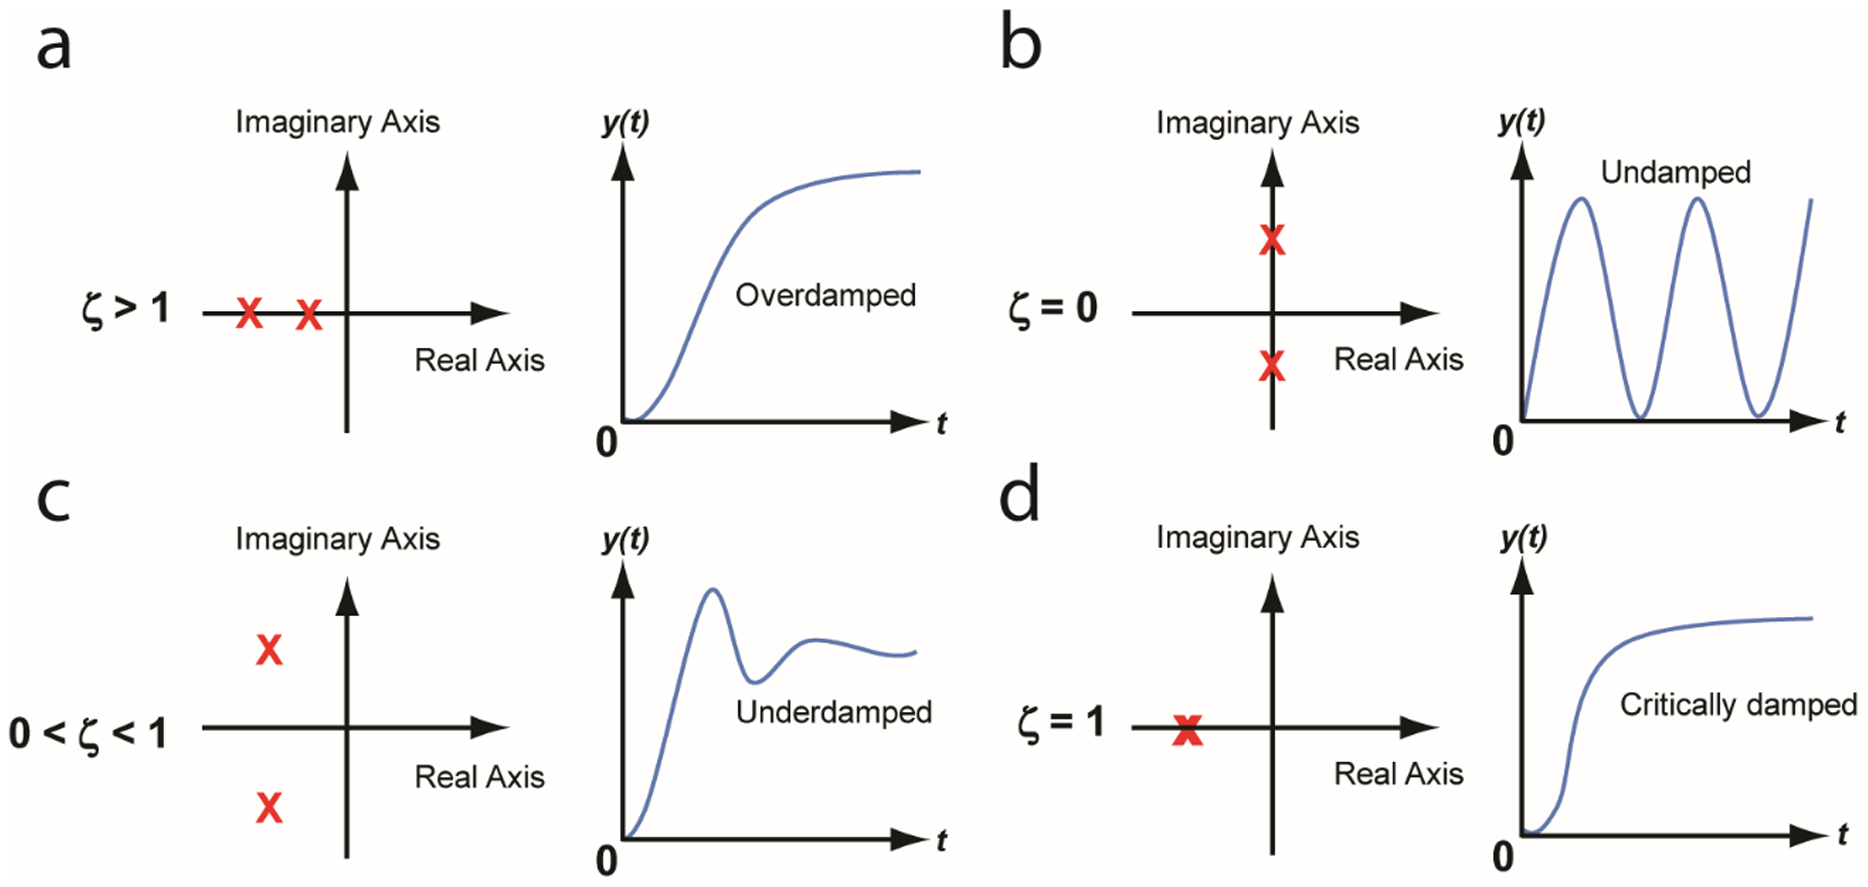
\includegraphics{img/damping.png}
\caption{Risposta Sistemi}
\end{figure}

    \hypertarget{analisi-generali-di-sistemi-di-2-ordine}{%
\subparagraph{Analisi generali di sistemi di 2°
ordine}\label{analisi-generali-di-sistemi-di-2-ordine}}

\begin{quote}
Un sistema di 2° ordine può essere caratterizzato mediante due grandezze
significative: \emph{la frequenza naturale} \(\omega_n\) e il fattore di
smorzamento \(\xi\). La frequenza naturale è la frequenza a cui
oscillerebbe il sistema non smorzato (undamped).
\end{quote}

Il fattore di smorzamento è definito come: \begin{equation}
\xi = \frac{\text{freq. decadimento esponenziale}}{\text{frequenza naturale}}
\end{equation}\\
o anche:\\
\begin{equation}
\xi = \frac{1}{2 \pi} \frac{\text{periodo naturale}}{\text{costante di tempo esponenziale}}
\end{equation}

    La formulazione generale di una funzione di trasferimento di 2° ordine
può quindi essere scritta come:\\
\begin{equation}
    G(s) = \frac{\omega^2_n}{s^2 + 2 \xi \omega_n s + \omega_n^2}
\end{equation}

    Si consulti la tabella a pagina 58. Molto importante.

    \hypertarget{calcolo-del-tempo-di-salita}{%
\subparagraph{Calcolo del tempo di
salita}\label{calcolo-del-tempo-di-salita}}

\begin{equation}
T_r = \frac{1 - 0.4167 \xi + 2.917 \xi^2}{\omega_n}
\end{equation}

\hypertarget{calcolo-del-tempo-di-setting}{%
\subparagraph{Calcolo del tempo di
setting}\label{calcolo-del-tempo-di-setting}}

\begin{equation}
T_s = \frac{- \ln\big(0.02 \sqrt{1-\xi^2}\big)}{\xi \omega_n}
\end{equation}

\hypertarget{calcolo-del-tempo-di-massimo-overshooting}{%
\subparagraph{Calcolo del tempo di massimo
overshooting}\label{calcolo-del-tempo-di-massimo-overshooting}}

\begin{equation}
T_p = \frac{\pi}{\omega_n \sqrt{1-\xi^2}}
\end{equation}

\hypertarget{calcolo-del-valore-di-os}{%
\subparagraph{Calcolo del valore di
\%OS}\label{calcolo-del-valore-di-os}}

\begin{equation}
\%OS = 100 \cdot \frac{y_{\text{max}} - y_{\text{finale}}}{y_{\text{finale}}}
\end{equation}

\begin{equation}
\%OS = 100\ e^{-\frac{\xi \pi}{\sqrt{1-\xi^2}}}
\end{equation}

\hypertarget{calcolo-di-xi}{%
\subparagraph{\texorpdfstring{Calcolo di
\(\xi\)}{Calcolo di \textbackslash{}xi}}\label{calcolo-di-xi}}

\begin{equation}
\xi = \frac{- \ln\big(\frac{\%OS}{100}\big)}{\sqrt{\pi^2 + \ln^2\big(\frac{\%OS}{100}\big)}}
\end{equation}


    % Add a bibliography block to the postdoc
    
    
    
    \end{document}
